
\begin{figure}
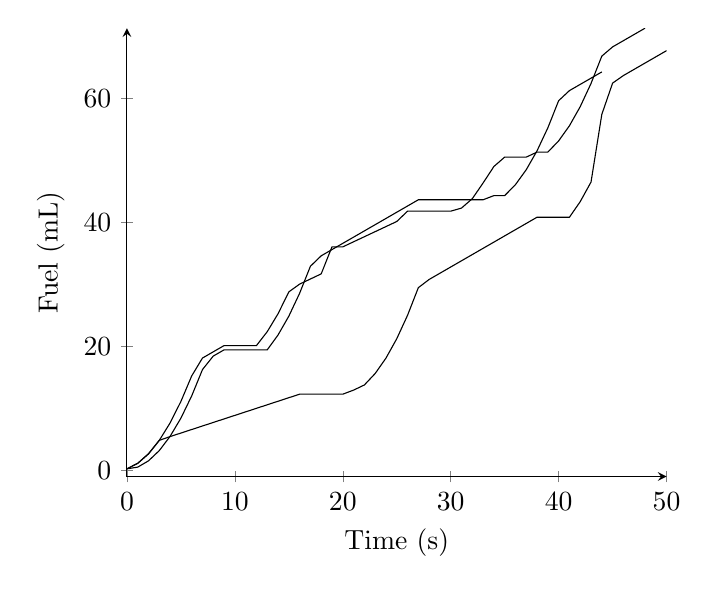
\begin{tikzpicture}
\begin{axis}[
legend style={anchor=west},
axis x line=bottom,
axis y line=left,
ymin=-1,
xlabel=Time (s),
ylabel=Fuel (mL),
]
\addplot[] coordinates {
(0, 0.239885513361)
(1, 1.13183007041)
(2, 2.66515136892)
(3, 4.83562037156)
(4, 7.64546130585)
(5, 11.1033516642)
(6, 15.2244222039)
(7, 18.1101790691)
(8, 19.1141689321)
(9, 20.1181587951)
(10, 20.1181587951)
(11, 20.1181587951)
(12, 20.1181587951)
(13, 22.362185017)
(14, 25.2462552635)
(15, 28.7797918319)
(16, 30.0306754741)
(17, 30.8570584212)
(18, 31.683704381)
(19, 36.0409523693)
(20, 36.0409523693)
(21, 36.8582408559)
(22, 37.6756894652)
(23, 38.4933514511)
(24, 39.31130509)
(25, 40.1296695882)
(26, 41.7943758465)
(27, 41.7943758465)
(28, 41.7943758465)
(29, 41.7943758465)
(30, 41.7943758465)
(31, 42.295732964)
(32, 43.8107428717)
(33, 46.3414518969)
(34, 48.9989805513)
(35, 50.5170378225)
(36, 50.5170378225)
(37, 50.5170378225)
(38, 51.3248611401)
(39, 51.3248611401)
(40, 53.1292286199)
(41, 55.5709009098)
(42, 58.6548460524)
(43, 62.3924853549)
(44, 66.8016933897)
(45, 68.2884131713)
(46, 69.2924030343)
(47, 70.2963928973)
(48, 71.3003827603)
};
\addplot[] coordinates {
(0, 0.239885513361)
(1, 1.13183007041)
(2, 2.66515136892)
(3, 4.83562037156)
(4, 5.44307886225)
(5, 6.0128261158)
(6, 6.58258022691)
(7, 7.15234304176)
(8, 7.72211710384)
(9, 8.29190600535)
(10, 8.86171496836)
(11, 9.43155184774)
(12, 10.0014289517)
(13, 10.5713665548)
(14, 11.1414002106)
(15, 11.7115975167)
(16, 12.2821018118)
(17, 12.2821018118)
(18, 12.2821018118)
(19, 12.2821018118)
(20, 12.2821018118)
(21, 12.9367467053)
(22, 13.768430324)
(23, 15.6140149187)
(24, 18.0970305264)
(25, 21.2228627952)
(26, 25.0033506385)
(27, 29.4567862341)
(28, 30.7825203723)
(29, 31.7865102353)
(30, 32.7905000984)
(31, 33.7944899614)
(32, 34.7984798244)
(33, 35.8024696874)
(34, 36.8064595504)
(35, 37.8104494135)
(36, 38.8144392765)
(37, 39.8184291395)
(38, 40.8224190025)
(39, 40.8224190025)
(40, 40.8224190025)
(41, 40.8224190025)
(42, 43.335235807)
(43, 46.4912778292)
(44, 57.4053862314)
(45, 62.45048895)
(46, 63.6685736522)
(47, 64.6725635152)
(48, 65.6765533783)
(49, 66.6805432413)
(50, 67.6845331043)
};
\addplot[] coordinates {
(0, 0.239885513361)
(1, 0.515724679301)
(2, 1.53163400129)
(3, 3.18760568115)
(4, 5.48065162036)
(5, 8.41423698528)
(6, 11.9982802071)
(7, 16.249152982)
(8, 18.4278188094)
(9, 19.4318086724)
(10, 19.4318086724)
(11, 19.4318086724)
(12, 19.4318086724)
(13, 19.4318086724)
(14, 21.8261981079)
(15, 24.8622712816)
(16, 28.5509716433)
(17, 32.9096959078)
(18, 34.5972233631)
(19, 35.6012132261)
(20, 36.6052030891)
(21, 37.6091929522)
(22, 38.6131828152)
(23, 39.6171726782)
(24, 40.6211625412)
(25, 41.6251524043)
(26, 42.6291422673)
(27, 43.6331321303)
(28, 43.6331321303)
(29, 43.6331321303)
(30, 43.6331321303)
(31, 43.6331321303)
(32, 43.6331321303)
(33, 43.6331321303)
(34, 44.3060855285)
(35, 44.3060855285)
(36, 46.0772777591)
(37, 48.4856928598)
(38, 51.5359627913)
(39, 55.2391727789)
(40, 59.612861313)
(41, 61.2389561315)
(42, 62.2429459945)
(43, 63.2469358575)
(44, 64.2509257205)
};

\end{axis}
\end{tikzpicture}
\label{tik:100:65}
\caption{100 percent diving with GSC on route $65$}
\end{figure}
